% ========== NILGÅS ==========
\begin{frame}{%
  \begin{minipage}[c]{0.30\textwidth}
    Nilgås
  \end{minipage}%
  \hfill
  \begin{minipage}[c]{0.45\textwidth}
    \footnotesize
    \textbf{Jagttid:} 1.\ sep. -- 31.\ jan. \\
    \textbf{Regulering:} Uden aftale: Hele året (invasiv)
  \end{minipage}%
  \hfill
  \begin{minipage}[c]{0.15\textwidth}
    \noindent\raggedleft
    
\includegraphics[width=0.5cm, height=0.5cm, keepaspectratio]{Billeder/Ikoner/star.png}
  \end{minipage}%
}
  \vspace{0.25em}
  \begin{columns}[T]
    % --- Venstre kolonne: Tekst ---
    \column{0.55\textwidth}
    \setlength{\parskip}{0.5em}
    \tiny
    \RaggedRight
    \textbf{\textit{Alopochen aegyptiaca}} – stor andelignende fugl som hverken er gås eller and \par
    \textbf{Udseende:}\\
    \quad – Begge: Broget med pletter rundt om øjnene
    % --- Højre kolonne: Ét billede ---
    \column{0.40\textwidth}
    \centering
    \fbox{%
      \begin{minipage}{\linewidth}
        \centering
        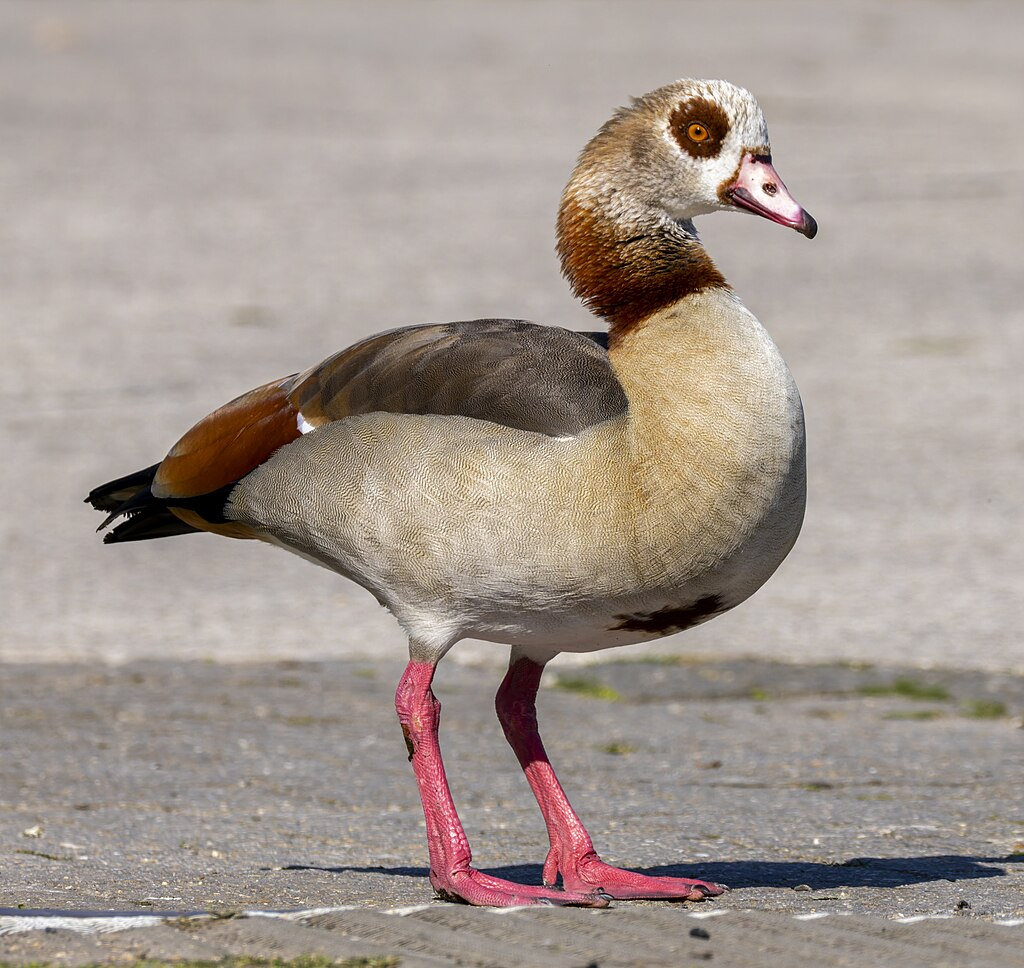
\includegraphics[width=0.85\linewidth, height=5.5cm, keepaspectratio]{Billeder/Dyr/Fugle/Aender/Gravaender/nilgås.jpg}
      \end{minipage}
    }%
  \end{columns}
\end{frame}